\section{Introduction}\label{sec:intro}

Online multiplayer games have the possibility of generating a lot of data, this increases with the possible options for each individual player and the number of players. 
\emph{League of Legends} (LoL), created by Riot games, was the most played online game in the beginning of 2015~\cite{LoLmostplayed}, mustering 27 million people playing it daily in the beginning of 2014~\cite{LoL27mill}. 

When playing, the players are divided into two competing teams, blue and purple, of 5 players each. In a classic match, each player will pick a champion (character) from a pool of 124 different champions, each with 4 unique abilities. An ability is a magic spell, which does widely different things, such as throwing a fireball at an opponent champion.

\begin{figure}[!htb]%{r}{{0.5\textwidth}} %Ikke sikker på jeg kan lide figure //Funder
  \centering
    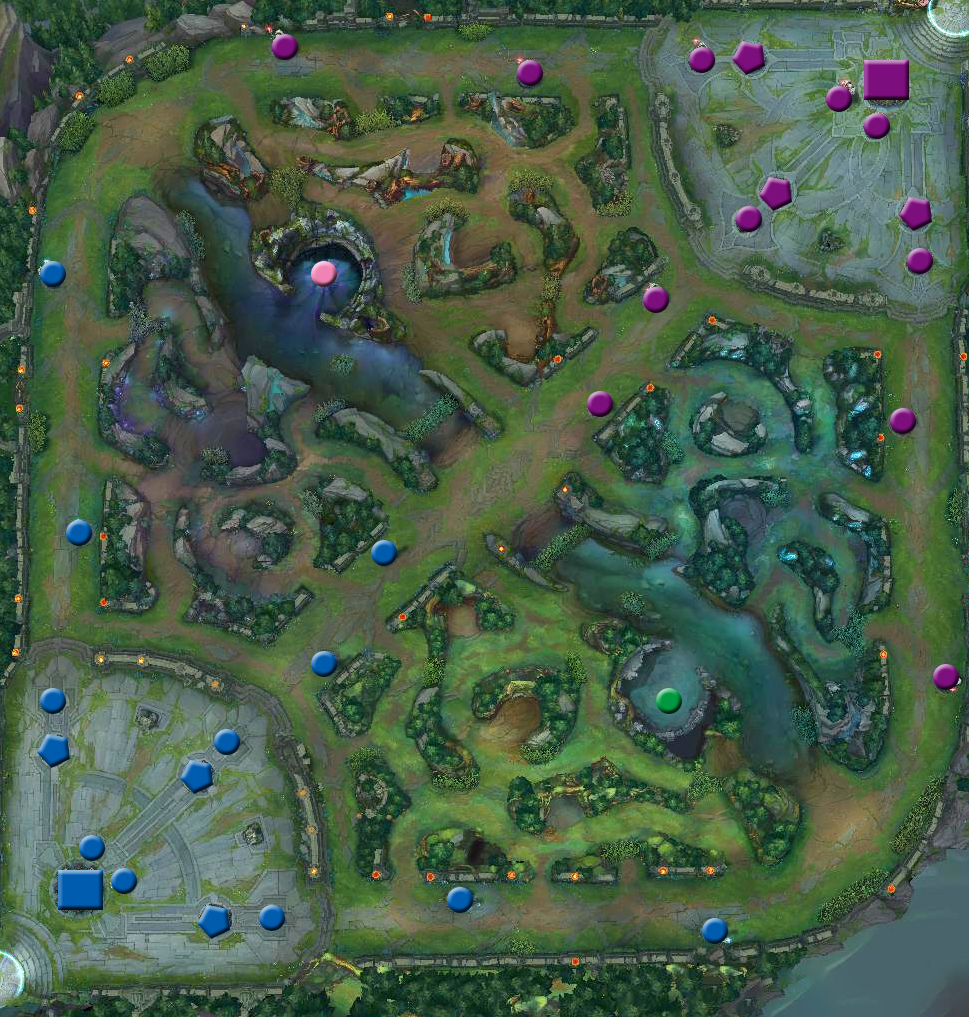
\includegraphics[width=0.5\textwidth]{img/lolmap.jpg}
  \caption{League of Legends map}\label{fig:lolmap}
\end{figure}

The map, seen in \Cref{fig:lolmap}, consists of three lanes, called \emph{top}, \emph{middle} and \emph{bottom} which connects the two bases. In the figure blue colors are the blue teams' structures and the same for purple. Circles are turrets, pentagons are inhibitors and squares are nexuses. The green circle is the dragon and the pink circle is the baron.

\begin{table}[!htb]
\begin{tabular}{l p{13cm}}
\textbf{Nexus}: & When destroyed ends the game, making the destroying team the winners\\
\textbf{Inhibitor}: & Spawns \emph{creeps}, small monsters with low damage and health, which walks toward the opposing base on the lane it was spawned\\
\textbf{Turret}: & A defensive structure, which fires at nearby enemies\\
\textbf{Jungle}: & Area between the lanes which hosts stronger monsters that award gold and experience\\
\end{tabular}
\end{table}

The effect of the inhibitors is that the two team's monsters meet in the middle, which is where the teams will be fighting, killing each others creeps and champions. When the inhibitor is destroyed, it makes the opposing team summon stronger minions on the lane it was destroyed. Lastly, killing the dragon award the killing team with a lot of gold, and killing the baron makes the champions stronger temporarily.

Experience and money is earned through out the game for the individual players, when killing monsters or opposing players. The experience is used to improve the skills of the champion while money is spend purchasing items, that will make the player stronger. This sums up the most important aspects of the game, and it is already quite clear how statespace the game hosts. This makes it extremely complex, and very interesting to analyse what can be done to improve ones gameplay. 

The game combines strategy, individual player skill, communication and team play. It is a massive skill showcase, but how important is strategy? In this paper we will investigate how much of an advantage one can get by making good strategic decisions, based on a large dataset of matches played.


